\documentclass[11pt]{article}
\usepackage[margin=1in]{geometry}
\usepackage{amsmath,amssymb}
\usepackage{graphicx}
\usepackage[hidelinks]{hyperref}

\title{Literature-Implied Status: Warped Cone Coarse Baum--Connes}
\author{FA/Banach run \texttt{fa\_banach\_001}}
\date{2026-06-14}

\begin{document}
\maketitle

\section*{Status}

This is a literature-implied partial answer packet, not an original proof from
the run.  Dru\c{t}u--Nowak, arXiv:1501.03473, conjectured that the coarse
assembly map is not surjective for warped cones arising from their
spectral-gap ghost-projection construction.  Kitsios--Schick--Vigolo,
arXiv:2504.21811, explicitly identify the Roe/Dru\c{t}u--Nowak conjecture and
prove the unified warped-cone non-surjectivity statement under the extra
hypotheses that the acting group has property A and the action is free and
strongly ergodic.

This does not settle the full 2015 conjecture, but it gives a direct
literature answer for an important natural subcase, including the standard
free-subgroup action on $\operatorname{SU}(2,\mathbb C)$ highlighted in the
supporting paper.

\section*{Original Problem}

The original source is:
\begin{quote}
C. Dru\c{t}u and P. W. Nowak, \emph{Kazhdan projections, random walks and
ergodic theorems}, arXiv:1501.03473.
\end{quote}

After proving that spectral-gap actions yield non-compact ghost projections
for warped cones, the paper states Conjecture 6.7: under the same hypotheses,
the coarse assembly map should not be surjective for the warped cone
$X=\mathcal O_G M$.

\begin{center}

\includegraphics[width=\textwidth]{figures/open_problem_crop.png}
\end{center}

\section*{Supporting Theorem}

The supporting source is:
\begin{quote}
C. Kitsios, T. Schick, and F. Vigolo, \emph{Coarse Baum-Connes and warped
cones: failure of surjectivity in odd degree}, arXiv:2504.21811.
\end{quote}

The 2025 paper formulates the relevant conjecture as Roe/Dru\c{t}u--Nowak
Conjecture 7.7 for a compact Riemannian manifold $M$ and a
measure-preserving action by diffeomorphisms with spectral gap.

\begin{center}
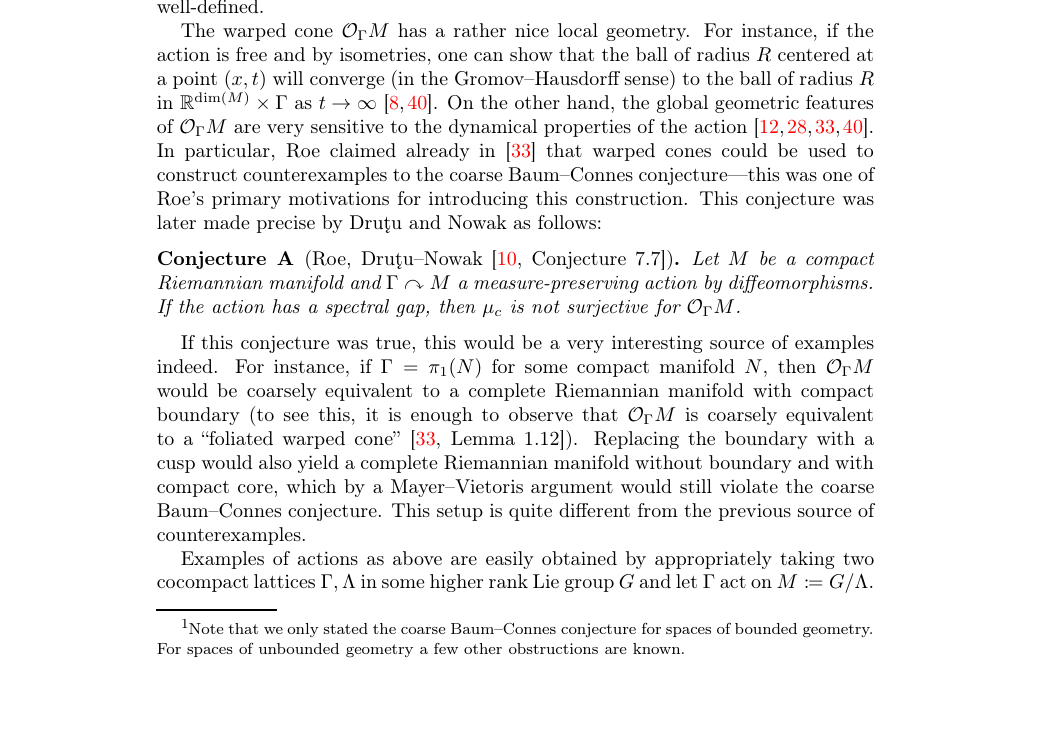
\includegraphics[width=\textwidth]{figures/supporting_conjecture_theorem_crop.png}
\end{center}

Its Theorem C says that if $\Gamma$ has property A and
$\Gamma\curvearrowright M$ is a free strongly ergodic action by
diffeomorphisms, then
\[
  \mu_c: KX_1(\mathcal O_\Gamma M)
    \longrightarrow K_1(C^*_{\mathrm{Roe}}(\mathcal O_\Gamma M))
\]
is not surjective.  The authors note that this does not exactly match the
Dru\c{t}u--Nowak conjecture: it adds property A and freeness, while replacing
spectral gap by the weaker strong ergodicity condition.  They also note that
their $\operatorname{SU}(2,\mathbb C)$ action satisfies the hypotheses.

\begin{center}
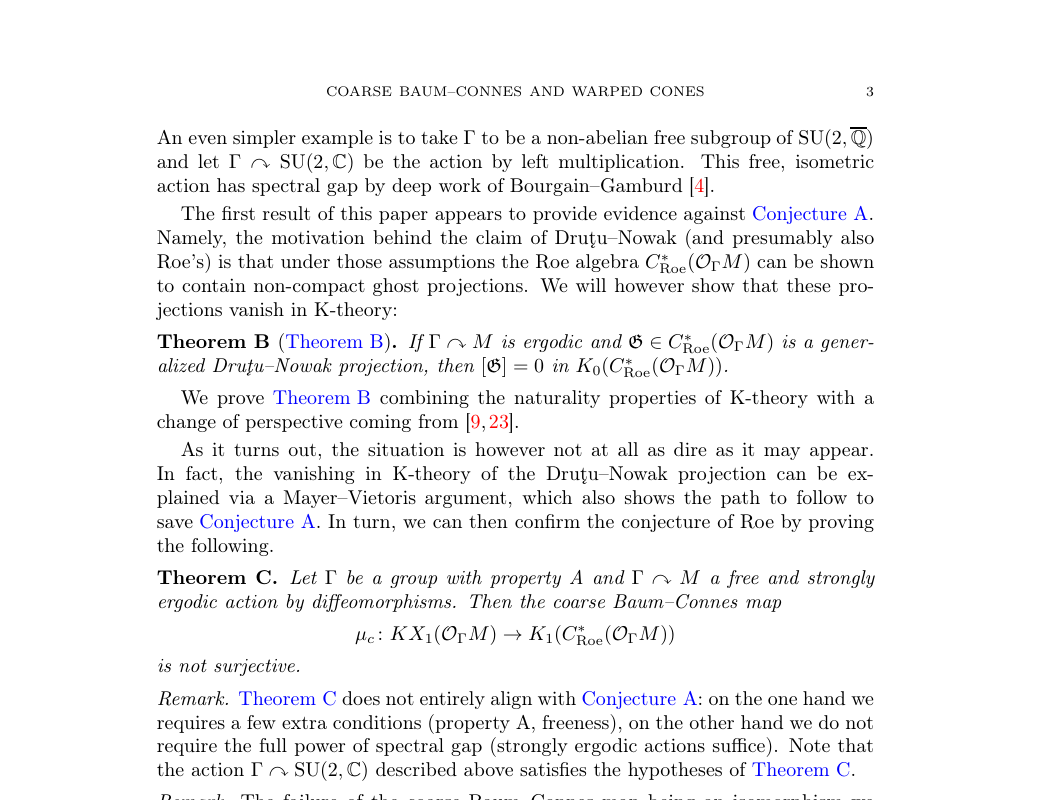
\includegraphics[width=\textwidth]{figures/supporting_theorem_c_crop.png}
\end{center}

\section*{Idea of the Supporting Proof}

The original Dru\c{t}u--Nowak route expected the non-compact ghost projection
itself to supply an even-degree $K$-theory obstruction.  Kitsios--Schick--
Vigolo show that generalized Dru\c{t}u--Nowak projections actually vanish in
$K_0$ for ergodic actions.  They then use a Mayer--Vietoris decomposition of
the unified warped cone and sparse-level ghost-projection obstructions to
produce an odd-degree class in the Roe algebra that cannot lie in the image of
the coarse assembly map.

\section*{Implication for arXiv:1501.03473}

For the property-A/free/strongly ergodic subcase, Kitsios--Schick--Vigolo give
the non-surjectivity conclusion sought by Dru\c{t}u--Nowak.  In particular,
spectral gap implies strong ergodicity for measure-preserving actions, and
free groups have property A, so the free-subgroup $\operatorname{SU}(2)$
examples fall within this supporting theorem.

\section*{Scope and Limitations}

This packet should be read as a literature-implied partial answer.  The full
statement of Conjecture 6.7 in arXiv:1501.03473 is broader: it does not impose
property A or freeness.  The 2025 theorem is therefore not a full
\texttt{literature\_already\_answered} resolution of the 2015 conjecture.

The scan hit quoting Willett--Yu Problem 5.4 is a same-paper
ask-and-answer passage: Dru\c{t}u--Nowak answer that older request by
constructing warped-cone ghost projections.  A nearby ``coarsely contain
expanders'' question in the source TeX is inside a discarded
\verb|\comment...\endcomment| block and was not treated as a published target.

\section*{References}

\begin{itemize}
\item C. Dru\c{t}u and P. W. Nowak, \emph{Kazhdan projections, random walks
and ergodic theorems}, arXiv:1501.03473.
\item C. Kitsios, T. Schick, and F. Vigolo, \emph{Coarse Baum-Connes and
warped cones: failure of surjectivity in odd degree}, arXiv:2504.21811.
\item K. Li, F. Vigolo, and J. Zhang, \emph{A Markovian and Roe-algebraic
approach to asymptotic expansion in measure}, arXiv:2008.12572, used only as
background for the sparse/integral warped-cone literature trail.
\end{itemize}

\section*{Review Recommendation}

Check the status label.  The packet records a real later-literature
confirmation for a major subcase and for the canonical $\operatorname{SU}(2)$
example, while preserving that the unrestricted spectral-gap conjecture is
not fully settled here.

\end{document}
